\chapter{Introdução}
\section{Objetivo}
  O objetivo deste projeto é comparar o desempenho de diferentes algoritmos de
ordenação em termos de tempo e espaço de execução, utilizando uma variedade de
conjuntos de dados.


\chapter{Metodologia}
\section{Resultados para DataSet Ordenado}

\begin{figure}[H]
  \centering
  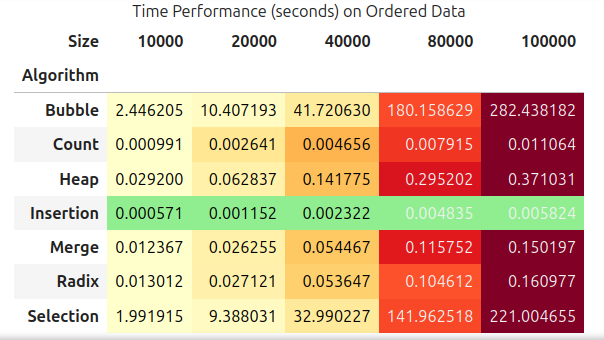
\includegraphics[width=0.6\textwidth]{images/order_table}
\end{figure}

\begin{figure}[H]
  \centering
  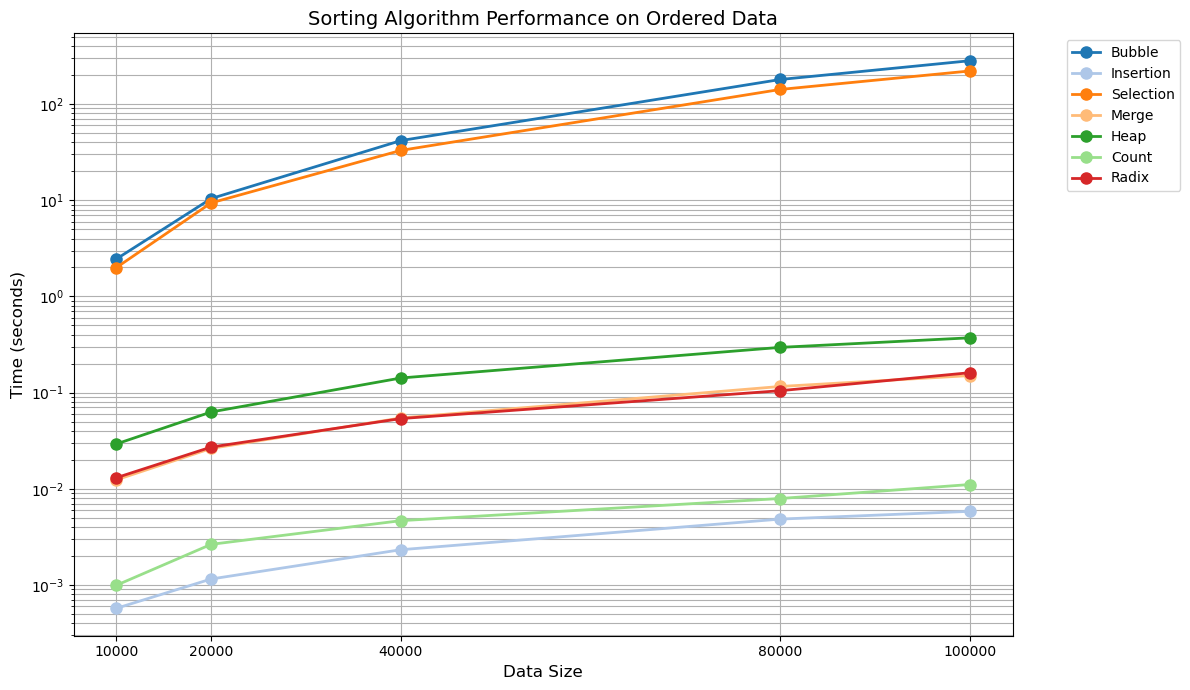
\includegraphics[width=0.6\textwidth]{images/all_algo_order}
\end{figure}

\begin{figure}[H]
  \centering
  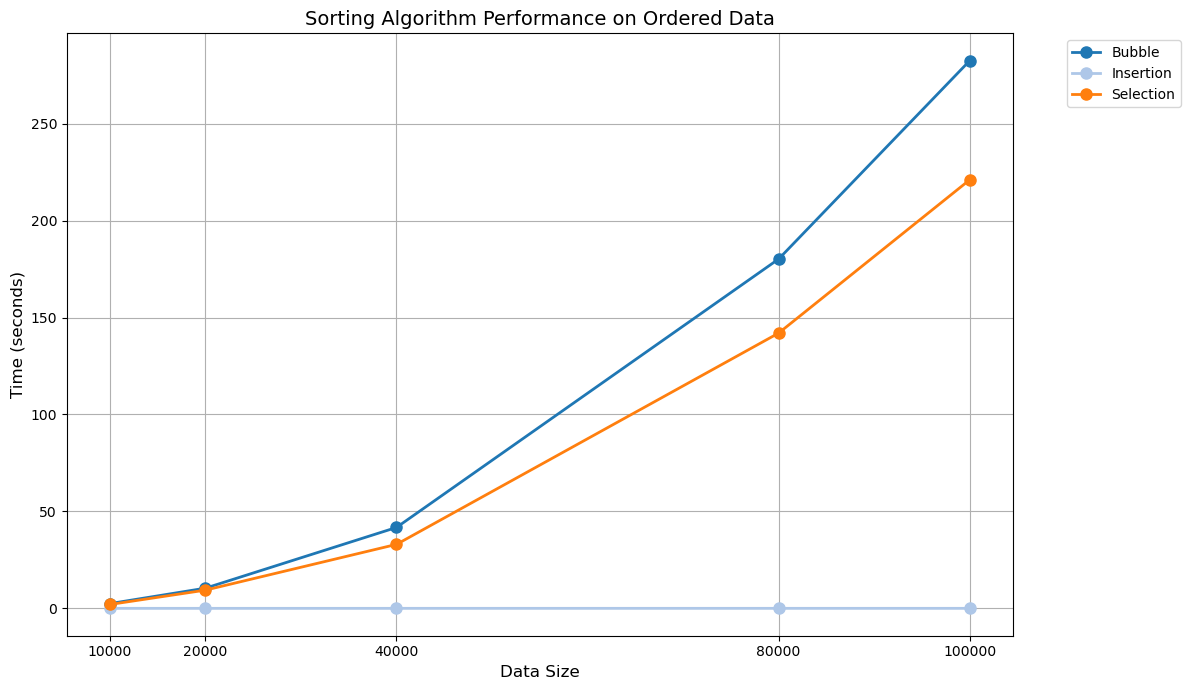
\includegraphics[width=0.6\textwidth]{images/o2_order}
\end{figure}

\begin{figure}[H]
  \centering
  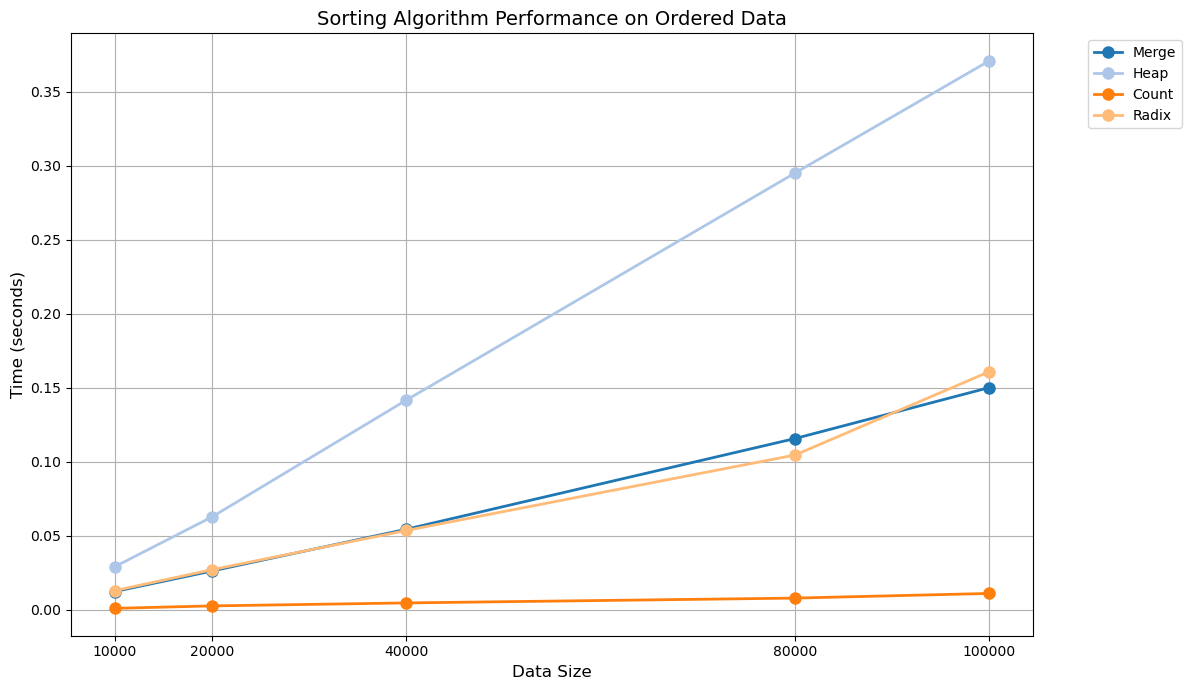
\includegraphics[width=0.6\textwidth]{images/o_order}
\end{figure}

\section{Resultados para DataSet Inversamente Ordenado}

\begin{figure}[H]
  \centering
  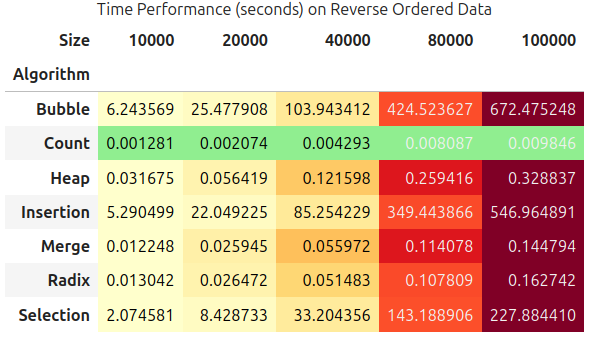
\includegraphics[width=0.6\textwidth]{images/invert_table}
\end{figure}

\begin{figure}[H]
  \centering
  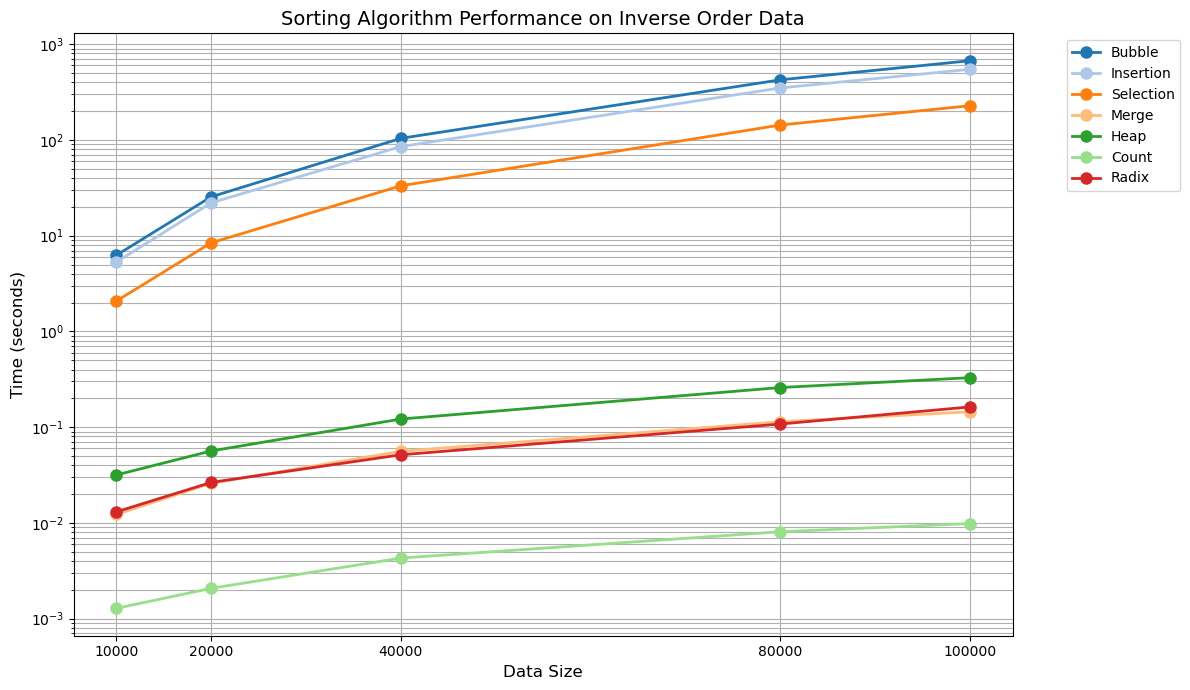
\includegraphics[width=0.6\textwidth]{images/all_algo_inver}
\end{figure}

\begin{figure}[H]
  \centering
  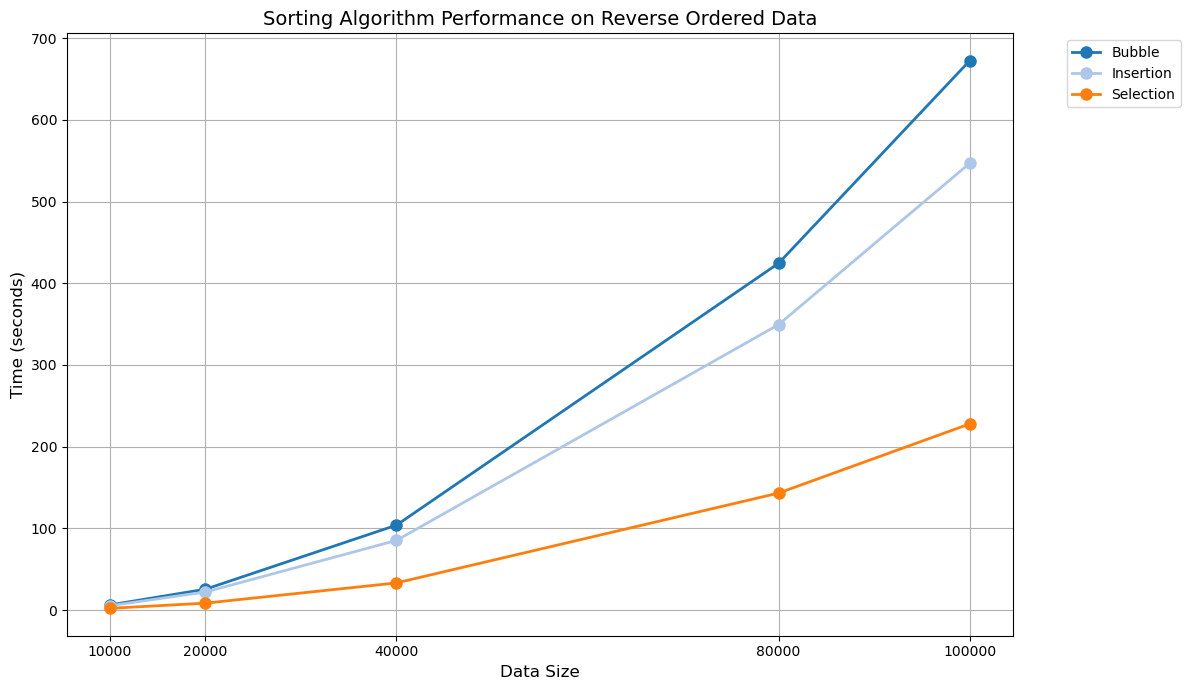
\includegraphics[width=0.6\textwidth]{images/o2_inv}
\end{figure}

\begin{figure}[H]
  \centering
  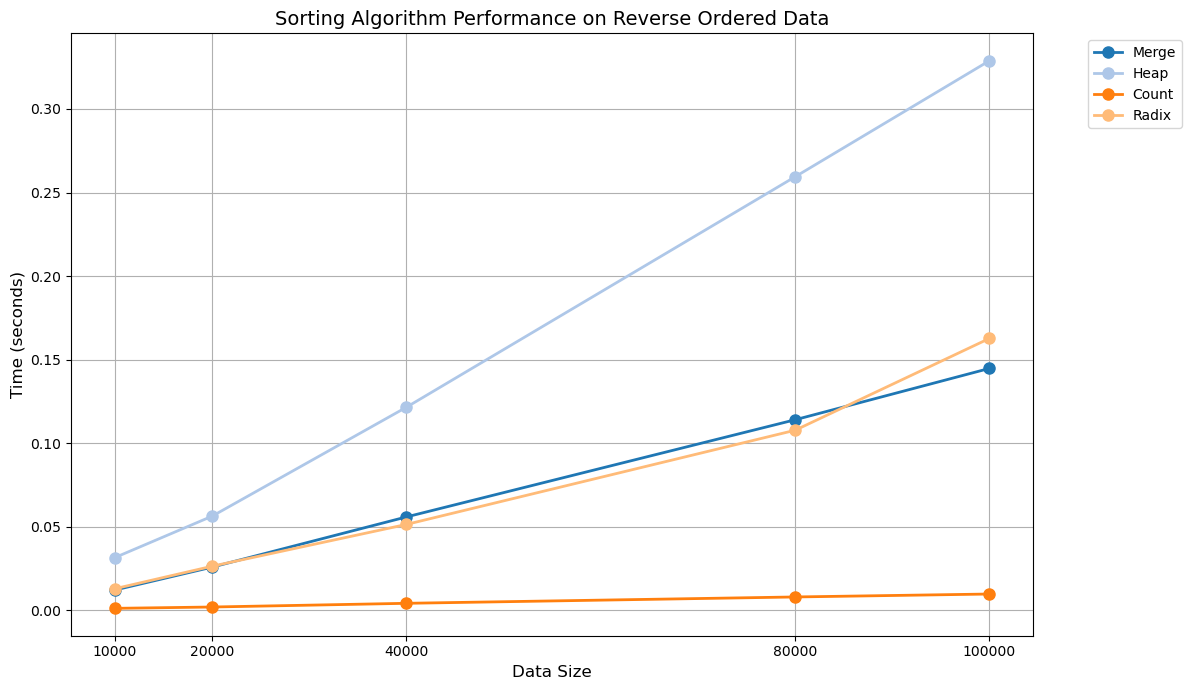
\includegraphics[width=0.6\textwidth]{images/o_inv}
\end{figure}

\section{Resultados para DataSet Aleatoriamente Ordenado}
\begin{figure}[H]
  \centering
  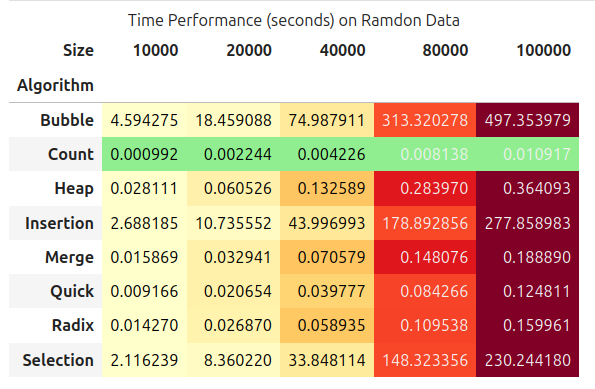
\includegraphics[width=0.6\textwidth]{images/random_table}
\end{figure}

\begin{figure}[H]
  \centering
  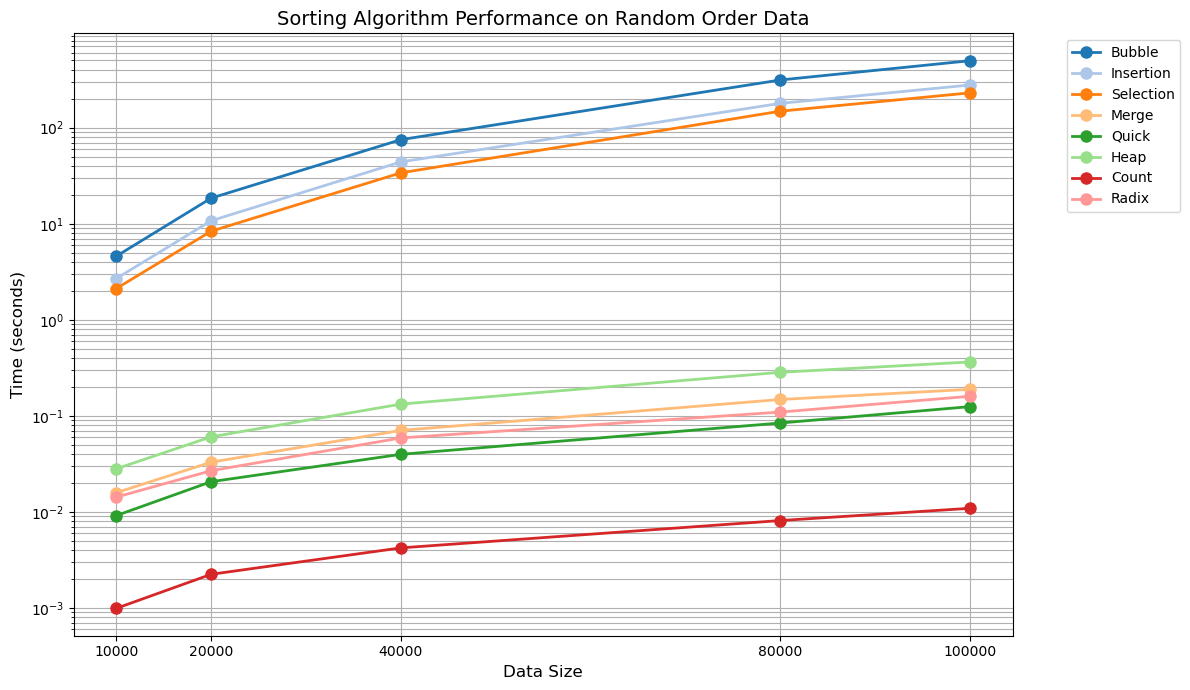
\includegraphics[width=0.6\textwidth]{images/all_algo_rand}
\end{figure}

\begin{figure}[H]
  \centering
  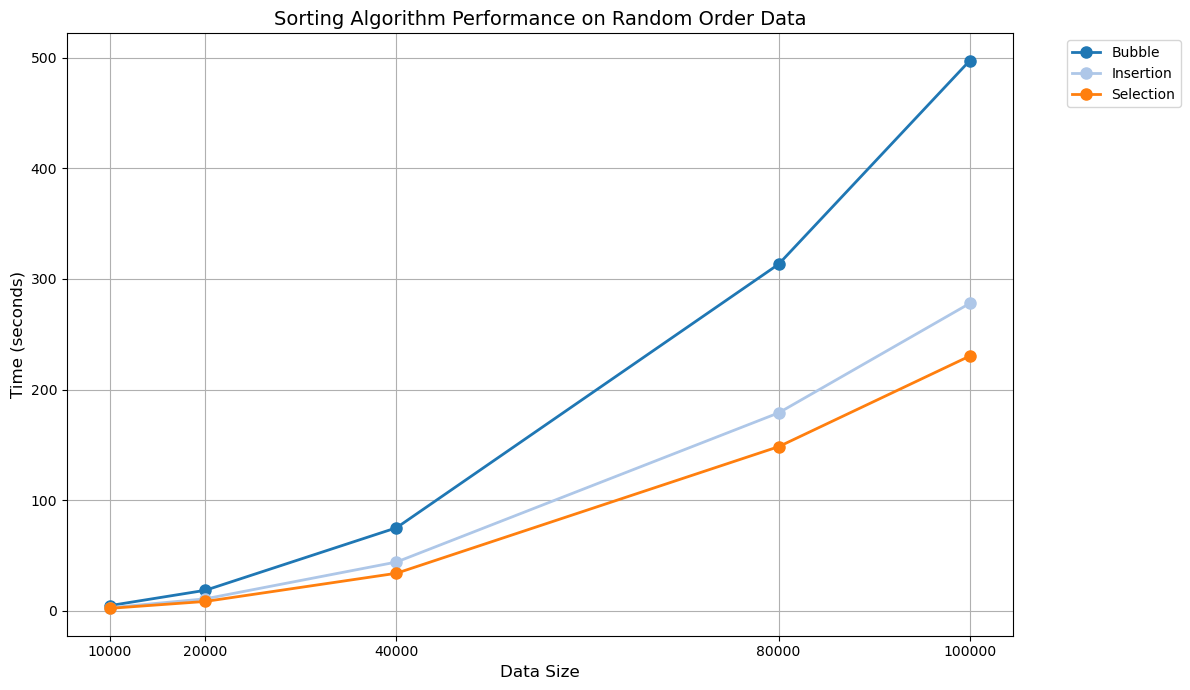
\includegraphics[width=0.6\textwidth]{images/o2_random}
\end{figure}

\begin{figure}[H]
  \centering
  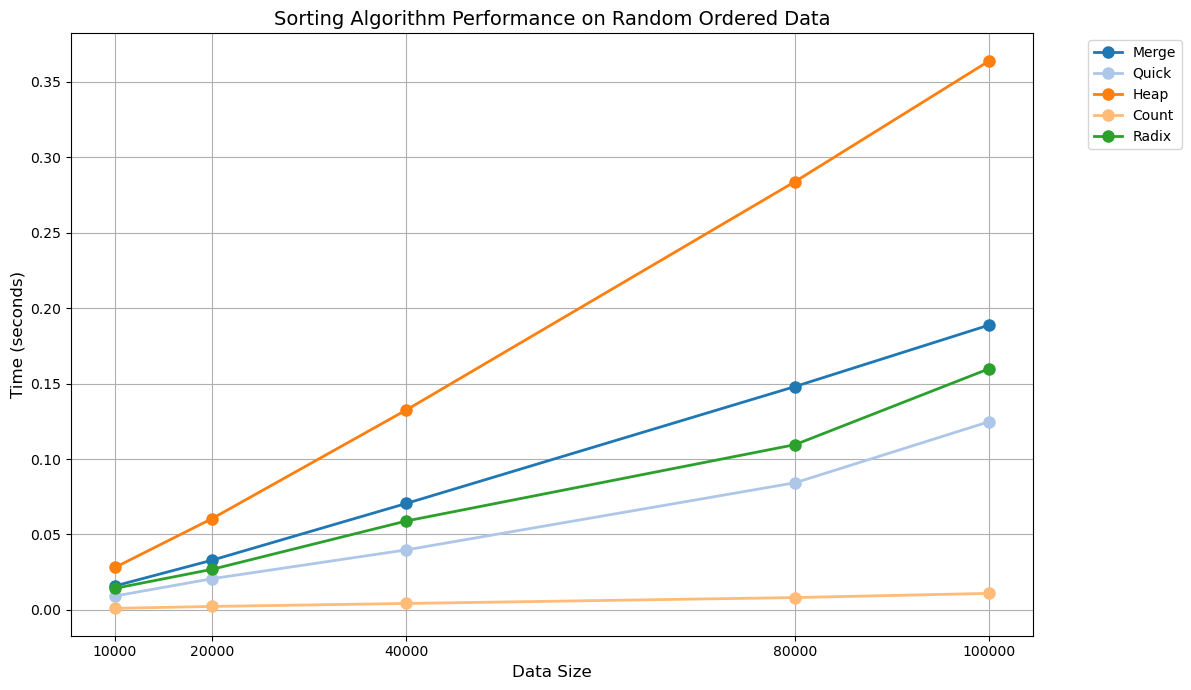
\includegraphics[width=0.6\textwidth]{images/o_random}
\end{figure}

\chapter{Conclusões}
